\subfigure{
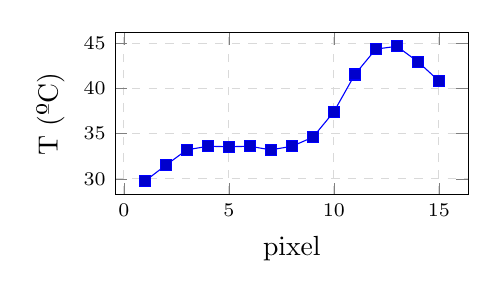
\begin{tikzpicture}
\begin{axis}[
	width=0.5\linewidth,
    height=0.3\linewidth,
	%title = {Processed Results},
    tick label style={font=\scriptsize},
    legend style={font=\scriptsize,/tikz/column 2/.style={column sep=5pt},},
    %legend columns=2,
    legend cell align=left,
	legend pos =south east,
    grid=major, % Display a grid
    grid style={dashed,gray!30}, % Set the style
    xlabel={pixel},
    ylabel={T (ºC)}, 
    %ymin = 0, ymax = 11200,
    %ytick={300,325,350,375,400,425,450,475,500,525},
    %yticklabels={300,325,350,375,400,425,450,475,500,525},
    %xmin = 400, xmax = 1500,
    %ytick={0,1600,...,11200},
    %yticklabel style={
    %    /pgf/number format/fixed,
    %    /pgf/number format/precision=5},
	%scaled y ticks=false,
    ]
\addplot+[mark=square*,blue]
coordinates {(	1	,	29.73	)
(	2	,	31.5	)
(	3	,	33.2	)
(	4	,	33.59	)
(	5	,	33.55	)
(	6	,	33.59	)
(	7	,	33.2	)
(	8	,	33.59	)
(	9	,	34.59	)
(	10	,	37.4	)
(	11	,	41.53	)
(	12	,	44.34	)
(	13	,	44.65	)
(	14	,	42.95	)
(	15	,	40.83	)
};
%\addlegendentry{}
\end{axis}
\end{tikzpicture}
}